
\documentclass[book, 16 pt, conference]{ieeeconf}  

                                           
\IEEEoverridecommandlockouts                              
                                                    
\overrideIEEEmargins

\usepackage{graphicx} 
\usepackage{bm}
\usepackage{listings}
\usepackage{listings}
\usepackage{color}

\definecolor{dkgreen}{rgb}{0,0.6,0}
\definecolor{gray}{rgb}{0.5,0.5,0.5}
\definecolor{mauve}{rgb}{0.58,0,0.82}

\lstset{frame=tb,
  language=Java,
  aboveskip=3mm,
  belowskip=3mm,
  showstringspaces=false,
  columns=flexible,
  basicstyle={\small\ttfamily},
  numbers=none,
  numberstyle=\tiny\color{gray},
  keywordstyle=\color{blue},
  commentstyle=\color{dkgreen},
  stringstyle=\color{mauve},
  breaklines=true,
  breakatwhitespace=true,
  tabsize=3
}
\newcommand{\uvec}[1]{\boldsymbol{\hat{\textbf{#1}}}}


\title{\LARGE \bf
Artículo de Investigación\\
Exportación y visualización de grafos
}

\author{Sebastián Medina Medina\\
Análisis y Diseño de Algoritmos\\
30 de Octubre de 2019
}


\begin{document}
\maketitle
\thispagestyle{empty}
\pagestyle{empty}


%%%%%%%%%%%%%%%%%%%%%%%%%%%%%%%%%%%%%%%%%%%%%%%%%%%%%%%%%%%%%%%%%%%%%%%%%%%%%%%%
\begin{abstract}

Artículo de Investigación acerca de la complejidad, tiempos y visualización de un conjunto de datos extraídos de la librería Snap (en específico el círculo social de Facebook). Los datos son presentados en forma de grafos y los formatos que se utilizaron fueron GraphML, GEXF, GDF y GraphSon. El programa de visualización que se utilizó fue Gephi.
 
\end{abstract}
%%%%%%%%%%%%%%%%%%%%%%%%%%%%%%%%%%%%%%%%%%%%%%%%%%%%%%%%%%%%%%%%%%%%%%%%%%%%%%%%

%%%%%%%%%%%%%%%%%%%%%%%%%%%%%%%%%%%%%%%%%%%%%%%%%%%%%%%%%%%%%%%%%%%%%%%%%%%%%%%%
\section{Grafos}

En esta investigación, se analizaron el conjunto de datos de Facebook que representa un círculo social, pero exportado en diferentes formatos como: GraphML, GEXF, GDF y GraphSon. Para poder exportar los grafos a los formatos antes mencionados, se programó un método individual en C++.

\subsection{GraphML}

GraphML es un formato sencillo que consiste en la descripción de las características de un grafo en un archivo. Estas características son: gráficos dirigidos, no dirigidos y mixtos; hipergrafías; gráficos jerárquicos; representaciones gráficas; referencias a datos externos; datos de atributos específicos de la aplicación; y analizadores livianos. $^{1}$  \\

Para el Grafo utilizado en el programa, solamente se específico su dirección, el nodo origen, el nodo destino y el ID del nodo. Ejemplo: edge id="e1" source="0" target="1"\\

Las actividades realizadas paso a paso fueron: \\

\begin{enumerate}
\item Se implementa el código que pueda exportar el grafo en el formato GraphML:
	\begin{enumerate}
	\item Se crea y abre un archivo con un nombre específico y un sufijo de texto (.graphml)
	\item Imprimir dentro del archivo los requisitos de la librería y del grafo (Si es directo o no)
	\item Implementación de un "For" para escribir los nodos
	\item Implementación de un "For" para escribir la arista, el nodo padre y el nodo hijo.
	\item Se cierra el archivo .graphml
	\end{enumerate}
\item Una vez creado, introducir en Gephi para visualizar el grafo: \\
\end{enumerate} 

\begin{center}
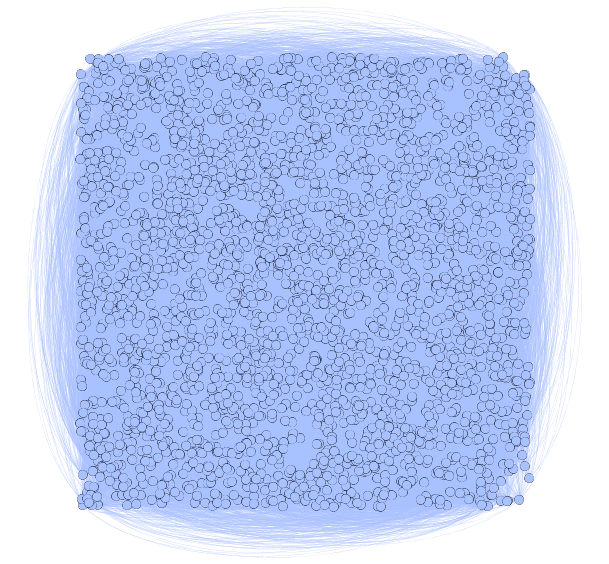
\includegraphics[scale=0.30]{1} 
\end{center}
FIG 1:(a) Grafo con el formato GraphML visualizado en Gephi.\\

La complejidad del algoritmo que exporta en formato GraphML es O(V + E) y el tiempo de ejecución del algoritmo fue de 174.902000 ms.

Las ventajas de utilizar el formato es que su tiempo de ejecución es menos de un segundo y el tiempo de visualizarlo igual es muy rápido.

\subsection{GDF}

GDF es el formato de archivo utilizado por GUESS. Está construido como una tabla de base de datos o un archivo separado por coma (CSV). Admite atributos tanto para nodos como para aristas. Un archivo estándar se divide en dos secciones, una para nodos y otra para bordes. Cada sección tiene una línea de encabezado, que básicamente es el título de la columna. Cada elemento (es decir, nodo o borde) está en una línea y los valores están separados por coma. Por lo tanto, el formato GDF es muy fácil de leer y se puede convertir fácilmente desde CSV. $^{2}$  \\

Las actividades realizadas paso a paso fueron: \\

\begin{enumerate}
\item Se implementa el código que pueda exportar el grafo en el formato GDF:
	\begin{enumerate}
	\item Se crea y abre un archivo con un nombre específico y un sufijo de texto (.gdf)
	\item Implementación de un "For" para escribir los nodos
	\item Implementación de un "For" para escribir la arista, el nodo padre
	\item Se cierra el archivo .gdf
	\end{enumerate}
\item Una vez creado, introducir en Gephi para visualizar el grafo: \\
\end{enumerate} 

\begin{center}
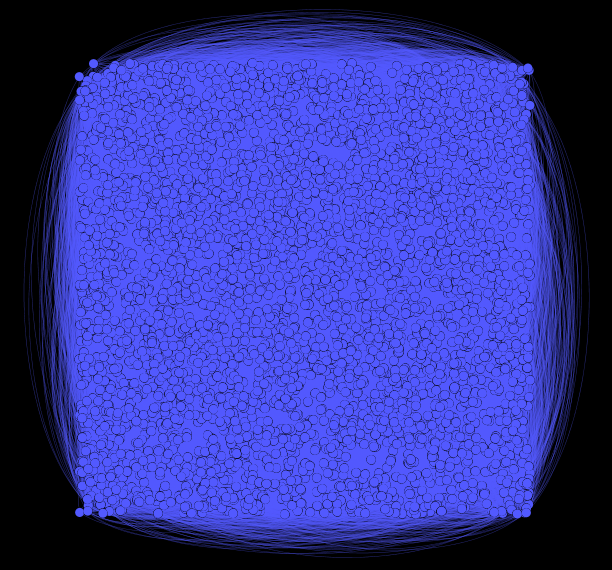
\includegraphics[scale=0.30]{2} 
\end{center}
FIG 2:(b) Grafo con el formato GDF visualizado en Gephi.\\

La complejidad del algoritmo que exporta en formato GDF es O(V + E) y el tiempo de ejecución del algoritmo fue de 54.060000 ms.

Las ventajas de utilizar el formato es que su tiempo de ejecución es el menor de todos (54 milisegundos), pero el tiempo para visualizarlo, es el que más se demoro.

\subsection{GEXF}

GEXF (Graph Exchange XML Format) es un lenguaje para describir estructuras de redes complejas, sus datos y dinámicas asociadas. Comenzado en 2007 en el proyecto Gephi por diferentes actores, profundamente involucrados en los problemas de intercambio de gráficos, las especificaciones gexf son lo suficientemente maduras como para afirmar que son extensibles y abiertas, y adecuadas para aplicaciones específicas reales. $^{3}$ \\

Las actividades realizadas paso a paso fueron: \\

\begin{enumerate}
\item Se implementa el código que pueda exportar el grafo en el formato GEXF:
	\begin{enumerate}
	\item Se crea y abre un archivo con un nombre específico y un sufijo de texto (.gexf)
	\item Implementación de un "For" para escribir los nodos
	\item Implementación de un "For" para escribir la arista, el nodo padre y el nodo hijo
	\item Se cierra el archivo .gexf
	\end{enumerate}
\item Una vez creado, introducir en Gephi para visualizar el grafo: \\
\end{enumerate} 

\begin{center}
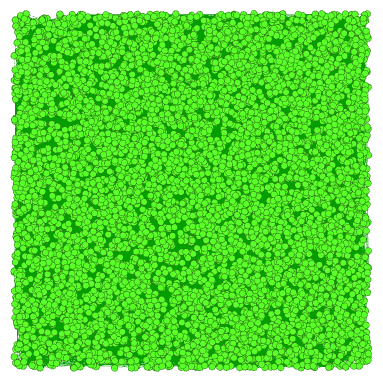
\includegraphics[scale=0.40]{3} 
\end{center}
FIG 3:(c) Grafo con el formato GEXF visualizado en Gephi.\\

La complejidad del algoritmo que exporta en formato GEXF es O(V + E) y el tiempo de ejecución del algoritmo fue de 178.904000 ms.

El algoritmo de exportación de GEXF es muy similar al de GraphML, ya que requieren la misma estructura, pero contienen diferentes requisitos, lo cual marca la diferencia del tiempo entre ambos algoritmos. Las ventajas de utilizar el formato es que su tiempo de ejecución es bajo y el tiempo de visualizarlo es bajo. 


\subsection{GraphSon}

GraphSON es un formato basado en JSON para elementos gráficos individuales (es decir, vértices y bordes). La forma en que estos elementos se organizan y utilizan cuando se escriben como un gráfico completo también se puede considerar en formato GraphSON. En otras palabras, el esquema para GraphSON es muy flexible y, por lo tanto, cualquier documento o fragmento JSON producido por los paquetes Blueprints IO puede ser considerado GraphSON válido. $^{4}$ \\

Para utilizar el formato JSON y poder graficarlo, de acuerdo a la documentación, debía existir un plugin que permitiera que exista una compatibilidad entre el programa Gephi y el formato graphson. Sin embargo, durante esta investigación, no se pudo visualizar el grafo mas si se pudo realizar el código.

Las actividades realizadas paso a paso fueron: \\

\begin{enumerate}
\item Se implementa el código que pueda exportar el grafo en el formato GraphSon:
	\begin{enumerate}
	\item Crear un archivo ".h" para implementar la escritura en el archivo. 
	\item Se crea y abre un archivo con un nombre específico y un sufijo de texto (.graphson)
	\item Implementación de un "For" para escribir los nodos.
	\item Implementación de un "For" para escribir la aristas.
	\item Se cierra el archivo .graphson
	\end{enumerate}
\end{enumerate} 

La complejidad del algoritmo que exporta en formato GraphSon es O(V + E) y el tiempo de ejecución del algoritmo fue de 621.330000 ms.

A pesar de tener una complejidad lineal, la demora del algoritmo deriva de la complejidad al escribir en el archivo, ya que necesita de más materiales a comparación con los otros algoritmos. 

El uso del formato Graphson tiene más desventajas que ventajas, ya que necesariamente se necesita un plugin para visualizarlo u otro visualizador mucho más complejo. La impresión en el archivo .graphson requiere de mayor tiempo de ejecución y más tiempo de programación. La ventaja del formato, es que te permite llenar más información como el peso y diferentes atributos al nodo (int, strings, boolean).

\section{Conclusión}

El programa para visualizar grafos, Gephi, fue muy útil para la investigación. El uso del programa es sencillo y muy amigable. No se necesita leer alguna documentación para aprender a usarlo a grandes rasgos. El programa te permite hacer diferentes funciones como ver la cantidad de nodos y aristas que el documento tiene, editar la forma de los nodos y aristas, ver la tabla detalladamente y poder agregar o eliminar nodos y aristas. Las desventaja del programa es que es muy lento cuando el grafo es muy grande y a veces no proyecta el grafo por falla del programa. En la instalación del programa pueden existir muchos problemas, pero la documentación te describe los pasos para solucionarlo. Otra desventaja es que no permite leer archivos JSON ni GraphSon.

\begin{thebibliography}{99}

\bibitem{c1} GraphML Team 2019. The GraphML File Format. (Enero 2019) Consultado: 30 de octubre de 2019 de http://graphml.graphdrawing.org/index.html.
\bibitem{c2} Gephi 2008-2017. GDF Format. Consultado: 30 de octubre de 2019 de https://gephi.org/users/supported-graph-formats/gdf-format/
\bibitem{c3} Gephi. GEXF File Format. Consultado: 30 de octubre de 2019 de https://gephi.org/gexf/format/
\bibitem{c4}  jbmusso 2016. GraphSON Reader and Writer Library. (Julio 2016) Consultado: 30 de octubre de 2019 de https://github.com/tinkerpop/blueprints/wiki/GraphSON-Reader-and-Writer-Library\\\\

\end{thebibliography}

\section{Códigos}

GDF

\begin{lstlisting}

void grafoGDF(PUNGraph G) {

  ofstream myfile;
  vector<int> nodos = obtenerVerticesOrdenados(G);
  TIntV conexiones;

  myfile.open("Facebook.gdf");

  myfile << "nodedef>name VARCHAR" << "\n";
  myfile << "edgedef>node1 VARCHAR,node2 VARCHAR" << "\n";

  myfile << "nodedef>id VARCHAR\n";
		for (PUNGraph::TObj::TNodeI NI = G->BegNI(); NI < G->EndNI(); NI++)
			myfile << NI.GetId() << "\n";

		myfile << "edgedef>source VARCHAR, destination VARCHAR\n";
		for (PUNGraph::TObj::TEdgeI EI = G->BegEI(); EI < G->EndEI(); EI++)
			myfile << EI.GetSrcNId() << ", " << EI.GetDstNId() << "\n";

  myfile.close();

}

\end{lstlisting}

GrapML

\begin{lstlisting}

void grafoML(PUNGraph G) {

  ofstream myfile;
  vector<int> nodos = obtenerVerticesOrdenados(G);
  TIntV conexiones;

  myfile.open("Facebook.graphml");

  myfile << "<?xml version=\"1.0\" encoding=\"UTF-8\"?>" << "\n";
  myfile << "<graphml xmlns=\"http://graphml.graphdrawing.org
  /xmlns\"" << "\n";
  myfile << "\txmlns:xsi=\"http://www.w3.org/2001/
  XMLSchema-instance\"" << "\n";
  myfile << "\txsi:schemaLocation=\"http://graphml.
  graphdrawing.org/xmlns/1.0/graphml.xsd\">" << "\n";
  myfile << "  <graph id=\"G\" edgedefault=\"undirected\">" << "\n";

  for (PUNGraph::TObj::TNodeI NI = G->BegNI(); NI < G->EndNI(); NI++)
			myfile << "<node id=\"" << NI.GetId() << "\"/>\n";

		int i = 1;
	for (PUNGraph::TObj::TEdgeI EI = G->BegEI(); EI < G->EndEI(); EI++, ++i)
		myfile << "<edge id=\"e" << i << "\" source=\"" << EI.GetSrcNId() << "\" target=\"" << EI.GetDstNId() << "\"/>\n";

  myfile << "  </graph>" << "\n";
  myfile << "</graphml>" << "\n";

  myfile.close();

}

\end{lstlisting}

GEXF

\begin{lstlisting}

void grafoGEXF(PUNGraph G) {

  ofstream myfile;
  vector<int> nodos = obtenerVerticesOrdenados(G);
  TIntV conexiones;

  myfile.open("Facebook.gexf");

  myfile << "<?xml version=\"1.0\" encoding=\"UTF-8\"?>" << "\n";
  myfile << "<gexf xmlns=\"http://www.gexf.net/1.2draft\" version=\"1.2\">" << "\n";
  myfile << "\t<graph mode=\"static\" defaultedgetype=\"undirected\">" << "\n";
  myfile << "\t\t<edges>" << endl;

  myfile << "<nodes>\n";
		for (PUNGraph::TObj::TNodeI NI = G->BegNI(); NI < G->EndNI(); NI++)
			myfile << "<node id=\"" << NI.GetId() << "\" />\n";
		myfile << "</nodes>\n";

		myfile << "<edges>\n";
		int i = 1;
		for (PUNGraph::TObj::TEdgeI EI = G->BegEI(); EI < G->EndEI(); EI++, ++i)
			myfile << "<edge id=\"" << i << "\" source=\"" << EI.GetSrcNId() << "\" target=\"" << EI.GetDstNId() << "\" />\n";
		myfile << "</edges>\n";

  myfile << "\t\t</edges>" << "\n";
  myfile << "\t</graph>" << "\n";
  myfile << "</gexf>" << "\n";

  myfile.close();

}

\end{lstlisting}

GraphSon

\begin{lstlisting}

GraphSONParser gson("Facebook");
    int nodeCounter = 0;
    int edgeCounter = 0;
    gson.initGraph();
    gson.initNodes();
    for(SnapNode NI = Graph->BegNI(); NI!=Graph->EndNI(); NI++)
    {
        nodeCounter++;
        if(nodeCounter == Graph->GetNodes())
            gson.writeNode(NI, true);
        else
            gson.writeNode(NI, false);
    }
    gson.closeNodes();
    gson.initEdges();
    for(SnapEdge EI = Graph->BegEI(); EI!=Graph->EndEI(); EI++)
    {
        edgeCounter++;
        if(edgeCounter == Graph->GetEdges())
            gson.writeEdge(EI, true);
        else
            gson.writeEdge(EI, false);
    }
    gson.closeEdges();
    gson.endGraph();

\end{lstlisting}

Link del código: https://github.com/tec-csf/tc2017-t4-otono-2019-sebastianmed

\end{document}
